% !TEX program = pdflatex
% Part 3 report skeleton. Same preamble and conventions as the Part 2 report.
% Red [TODO] marks work or numbers still to fill in. Figures go in img/.
\documentclass[10pt,letterpaper]{article}
\usepackage[T1]{fontenc}
\usepackage{lmodern,amsmath,amssymb,booktabs,graphicx,microtype,array,tabularx}
\usepackage[margin=.75in,headheight=14pt]{geometry}
\usepackage{subcaption,float,xcolor,fancyhdr,colortbl,tikz}
\usetikzlibrary{arrows.meta,automata,positioning}
\usepackage[colorlinks=true,linkcolor=blue!40!black,urlcolor=blue!40!black]{hyperref}
\definecolor{navy}{HTML}{153654}\definecolor{pale}{HTML}{EAF1F7}
\definecolor{okc}{HTML}{DDF3DD}\definecolor{partc}{HTML}{FFF2CC}\definecolor{missc}{HTML}{F8D7D7}
\setlength{\parindent}{0pt}\setlength{\parskip}{4pt}
\graphicspath{{img/}}
\pagestyle{fancy}\fancyhf{}\fancyhead[L]{\small ESE 5700 / Project 1 / Part 3}\fancyhead[R]{\small MAC unit}\fancyfoot[C]{\thepage}\renewcommand{\headrulewidth}{.3pt}
\captionsetup{font=small,labelfont=bf,skip=3pt}
\newcommand{\todo}[1]{\textcolor{red}{\textbf{[TODO: #1]}}}
\newcommand{\est}{\textit{(est.)}}
\newcommand{\code}[1]{\texttt{#1}}
\newcommand{\fig}[3]{\begin{figure}[H]\centering\IfFileExists{img/#1.png}{\includegraphics[width=#2\linewidth]{#1}}{\fbox{\parbox{.6\linewidth}{\centering\small\textcolor{red}{[missing figure: \detokenize{#1}]}\vspace{1.2cm}}}}\caption{#3}\end{figure}}
\newcommand{\rub}[2]{\par\noindent\fcolorbox{navy}{pale}{\parbox{.975\linewidth}{\small\textbf{Rubric (#1):} #2}}\par\smallskip}
\begin{document}
\begin{center}
{\small UNIVERSITY OF PENNSYLVANIA \quad ESE 5700}\par\vspace{4pt}
{\LARGE\bfseries Project 1, Part 3: the MAC unit}\par\vspace{3pt}
Tyrone Marhguy \quad\textbullet\quad Victor Wanjohi \quad\textbullet\quad Due 10/27/2026\par\vspace{4pt}
\colorbox{pale}{\parbox{.95\linewidth}{\small\centering Cadence GPDK 18 nm \quad $V_{DD}=0.8$ V, nominal corner, 27$^\circ$C \quad $T_{CLK,\min}=\todo{ns}$ \quad 17 cycles START$\to$DONE (predicted) \quad area $\approx292\ \mu$m$^2$ \est}}
\end{center}

%==============================================================
\section*{Rubric map (handout, Part 3: ``Report'' list and 5-point grading)}
\begin{tabularx}{\linewidth}{@{}p{.5\linewidth}p{.07\linewidth}p{.13\linewidth}X@{}}
\toprule Required item & Pts & Section & Status\\\midrule
\rowcolor{missc}Register cell with its characterization (setup, hold, $t_{cq}$, $C_{CLK}$, energy per clock) & 1 & \S2 & \textbf{Missing}: cell designed and fixed; \code{tb\_dff} not run\\
\rowcolor{partc}Multiplier and adder schematics with sizes; logical-effort sizing of the critical path & 1.5 & \S3 & \textbf{Partial}: multiplier verified (256 pairs), delay bounded; schematics and logical effort missing\\
\rowcolor{partc}State diagram, sequencer schematic, one-dot-product timing diagram & 1.5 (with timing closure) & \S4 & \textbf{Partial}: state diagram and logic described from the netlist; schematics, benches, timing diagram missing\\
\rowcolor{missc}Timing closure: hand-computed critical path vs.\ measured $T_{CLK,\min}$; hold check & (above) & \S5 & \textbf{Missing}: critical path named; numbers need \S2 and \code{tb\_top}\\
\rowcolor{missc}Verification waveforms (Test A) and pass/fail table & 1 (with metrics and report quality) & \S6 & \textbf{Missing}: \code{tb\_top} not built\\
\rowcolor{partc}Metrics table: FOM$_{MAC}$, $D$, $V_{DD}$; energy per MAC with and without memory; where the energy goes & (above) & \S7 & \textbf{Partial}: area estimated; delay, energy, FOM missing\\
\rowcolor{partc}Short paragraph: what limited the design & & \S8 & \textbf{Partial}: first draft; final numbers missing\\
\rowcolor{partc}Top-level block diagram and schematic; team members and contributions & & \S1 & \textbf{Partial}: \code{top} schematic in; block diagram and contributions missing\\\bottomrule
\end{tabularx}
\smallskip
{\small Update the status colors (red missing, yellow partial, green done) as sections fill in. All simulations are schematic level (no extracted parasitics): bitline capacitance $C_{BL}=3.5$ fF per bitline (\code{cbw}, as in Part 2), and each block output under test drives one \code{inv\_2x}. Strategy from the handout: treat the SRAM as a black box with the Part 2 interface and $t_{access}$; register first, then the multiplier (exhaustive, all 256 pairs), then the accumulator, then the sequencer; simulate the full unit only when every piece passes alone.}

%==============================================================
\section*{1. Team members and contributions}
\begin{tabularx}{\linewidth}{@{}lX@{}}\toprule Member & Contribution\\\midrule
Victor Wanjohi & \todo{fill in}\\
Tyrone Marhguy & \todo{fill in}\\\bottomrule\end{tabularx}

\paragraph{Summary.} Two copies of the Part 2 macro hold the weights $W$ and activations $X$; a static-CMOS array multiplier, a 12-bit ripple-carry accumulator, a 4-bit address counter and a two-bit controller (all registers are transmission-gate master-slave flip-flops) compute $\mathrm{ACC}=\sum_{i=0}^{15}W[i]\,X[i]$. The read is pipelined against the multiply-accumulate (read in cycle $n$, accumulate in $n+1$), so a dot product takes 17 cycles from the START edge to DONE (cycle-level model of the netlist). The multiplier is correct for all 256 input pairs and its worst case is above 1.05 ns, so it, not the 488 ps SRAM read, sets the clock period. Area $\approx292\ \mu$m$^2$ \est. \todo{$T_{CLK,\min}$, Tests A/B/C result, energy.}

\fig{mac_top_schematic}{.98}{\code{top}, left half: the two \code{sram\_macro} instances (I1 weights, written when LOAD\_EN$\cdot$WE\_W; I0 activations, LOAD\_EN$\cdot$WE\_X), sharing MEM\_ADDR, CLK and DIN; their DOUT buses feed \code{multiplier4b} (I2), whose product feeds \code{accumulator\_12b} (I3). Top: LOAD\_EN $=\overline{\mathrm{RUN}+\mathrm{DONE}+\mathrm{START}}$ (two \code{or2}, \code{inv\_2x}).}
\fig{mac_top_schematic_right}{.98}{\code{top}, right half: \code{controller\_mac} (I5) and \code{counter\_4b} (I4) in a loop (COUNT\_EN, CLEAR, COUNT$\langle3{:}0\rangle$), and four \code{mux2} that send COUNT to MEM\_ADDR while RUN $=1$ and the external ADDR otherwise.}
\fig{mac_top_pins}{.6}{\code{top} ports: CLK, RST, START, ADDR$\langle3{:}0\rangle$, DIN$\langle3{:}0\rangle$, WE\_W, WE\_X in; DONE and ACC$\langle11{:}0\rangle$ out; VDD, VSS.}

\paragraph{Block inventory and test benches.}
\begin{center}\small\begin{tabular}{@{}llll@{}}\toprule Block & Built from & Test bench & Status\\\midrule
Register bit (DFF) & latch pair, T-gates & \code{tb\_dff} & designed; hold-loop bug fixed; not simulated\\
4$\times$4 multiplier & AND array, adders & \code{tb\_multiplier4b} & 256/256 correct; delay $>1.05$ ns (sweep to redo)\\
12-bit accumulator & adder 12b, 12 registers & \code{tb\_accu\_12b} & not simulated\\
4-bit counter & 4 DFFs, toggle chain & \code{tb\_counter4b} & stimulus and expected values ready\\
Controller (idle/compute/done) & 4 registers, gates & \code{tb\_controller} & stimulus and expected values ready\\
MAC top & all of the above and 2 macros & \code{tb\_top} & not built\\\bottomrule\end{tabular}\end{center}

%==============================================================
\section*{2. Sequential elements (3.1)}
\rub{3.1}{register bit at transistor level, used for accumulator, counter, controller state, DONE; setup, hold, clock-to-Q with the simulation that determines each; clock-input capacitance; energy per clock; style justified.}

\textbf{Style and justification.} Positive-edge master-slave flip-flop built from two static transmission-gate latches (\code{dlatch}): the master is transparent while CLK $=0$, the slave while CLK $=1$, so $D$ is captured on the rising edge. Each latch has an input \code{tg}, a storage node driven by two \code{inv\_2x}, a hold \code{tg} that closes the loop from $Q$, and its own clock inverter; the flip-flop adds one more \code{inv\_2x} to make the master's clock (100 fins: \code{tg} 2$+$2 fins, \code{inv\_2x} 8/4 fins). It was chosen because it reuses the verified \code{tg} and inverter cells, is fully static (holds with the clock stopped, unlike a dynamic C$^2$MOS latch), and needs only the single external clock. Its cost is the local clock inverters (clock load, and a small skew between the two phases, which hold must cover). \code{register\_1b} adds a \code{mux2} load enable ($EN=1$ loads $D$, $EN=0$ recirculates $Q$) and an \code{and2} synchronous reset (152 fins). \todo{Alternative considered (e.g.\ C$^2$MOS or pulsed latch) and why rejected, with numbers once \code{tb\_dff} has run.}

\textbf{Design note.} The first \code{dlatch} fed the node after one inversion back through the hold gate, an inverting loop that cannot store a value; the hold \code{tg} now returns $Q$ (two inversions) to the storage node and conducts while CLK $=0$ (fixed 10/25, before any register simulation).
\fig{dff_schematic}{.75}{\code{d\_ff}: master \code{dlatch} I0 clocked by CLKB (transparent while CLK $=0$), slave I1 clocked by CLK, and the clock inverter I2 (\code{inv\_2x}, 8/4 fins). Each \code{dlatch}: input and hold \code{tg} (2$+$2 fins), two \code{inv\_2x} in the loop and one for its local clock; 100 fins in total.}

\textbf{Test bench} (\code{tb\_dff}): \todo{D swept relative to the CLK edge, loaded by one register input or FO4, realistic input slews. Describe the bisection or sweep.}

\begin{center}\small\begin{tabular}{@{}p{.3\linewidth}p{.22\linewidth}p{.4\linewidth}@{}}\toprule Quantity & Value & Determined by\\\midrule
Setup time $t_{su}$ (D 0$\to$1 / 1$\to$0) & \todo{ps} & \todo{D-to-CLK offset at which Q fails, or CLK-to-Q rises by 10\% (state the criterion)}\\
Hold time $t_{h}$ & \todo{ps} & \todo{same criterion, D changing after the edge}\\
Clock-to-Q $t_{cq}$ (rise / fall) & \todo{ps} & \todo{CLK 50\% to Q 50\%, D stable well before the edge}\\
Clock-input capacitance $C_{CLK}$ & \todo{fF} & \todo{charge per cycle from CLK source / $V_{DD}$, or AC method}\\
Energy per clock & \todo{fJ} & \todo{integral of $V_{DD}$ current over one cycle, with D toggling / not toggling}\\\bottomrule\end{tabular}\end{center}
\fig{tb_dff_setup_sweep}{.7}{\todo{Setup-time determination: $t_{cq}$ against D-to-CLK offset, showing the wall.}}
\fig{tb_dff_hold_sweep}{.7}{\todo{Hold-time determination.}}
\fig{tb_dff_tran}{.7}{\todo{Clock-to-Q transient and the energy measurement window.}}

%==============================================================
\section*{3. Datapath (3.2)}
\rub{3.2}{4$\times$4 unsigned multiplier and 12-bit accumulator adder; any architecture justified; critical path sized with logical effort before simulating.}

\textbf{Leaf cells.} Static CMOS throughout, $L=18$ nm: \code{tg} (2+2 fins), \code{mux2} (two \code{tg} and an \code{inv\_2x}, $Y=S\,?\,B:A$), \code{xor2} (complementary static gate with input inverters, 44 fins), \code{and2} (\code{nand2\_u}$+$\code{inv\_2x}), \code{or2} (NOR2$+$\code{inv\_2x}). The full adder is $S=(A\oplus B)\oplus C_{in}$, $C_{out}=C_{in}(A\oplus B)+AB$ from two \code{xor2}, two \code{and2} and an \code{or2} (148 fins).
\begin{figure}[H]\centering
\IfFileExists{img/tgate_schematic.png}{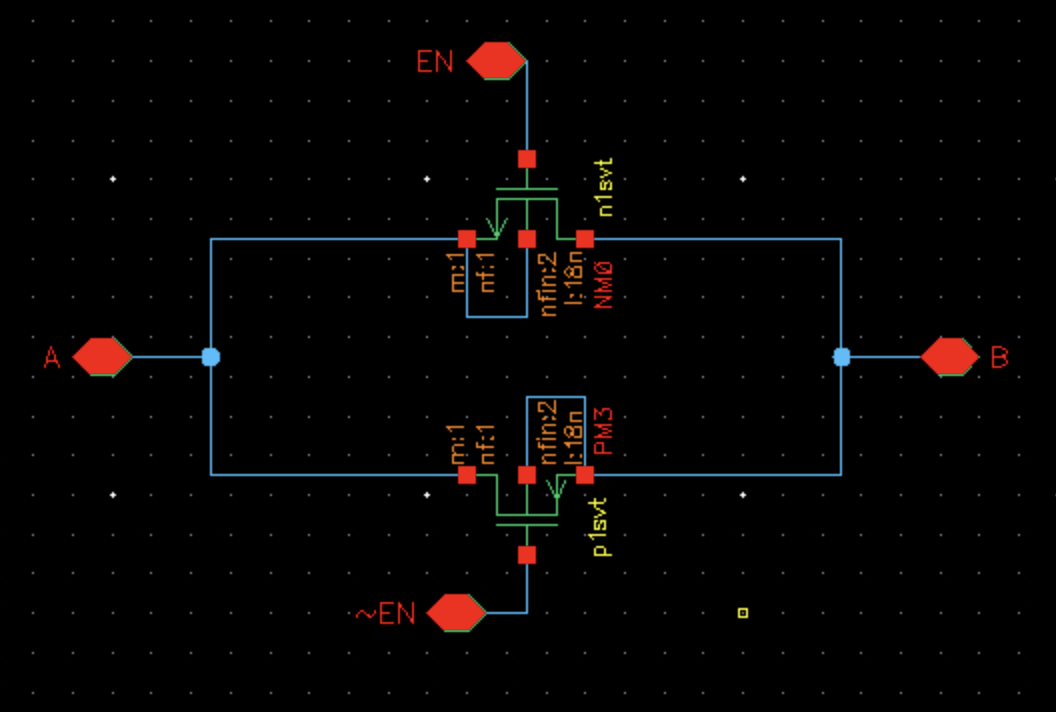
\includegraphics[width=.32\linewidth]{tgate_schematic}}{}\hfill
\IfFileExists{img/xor2_schematic.png}{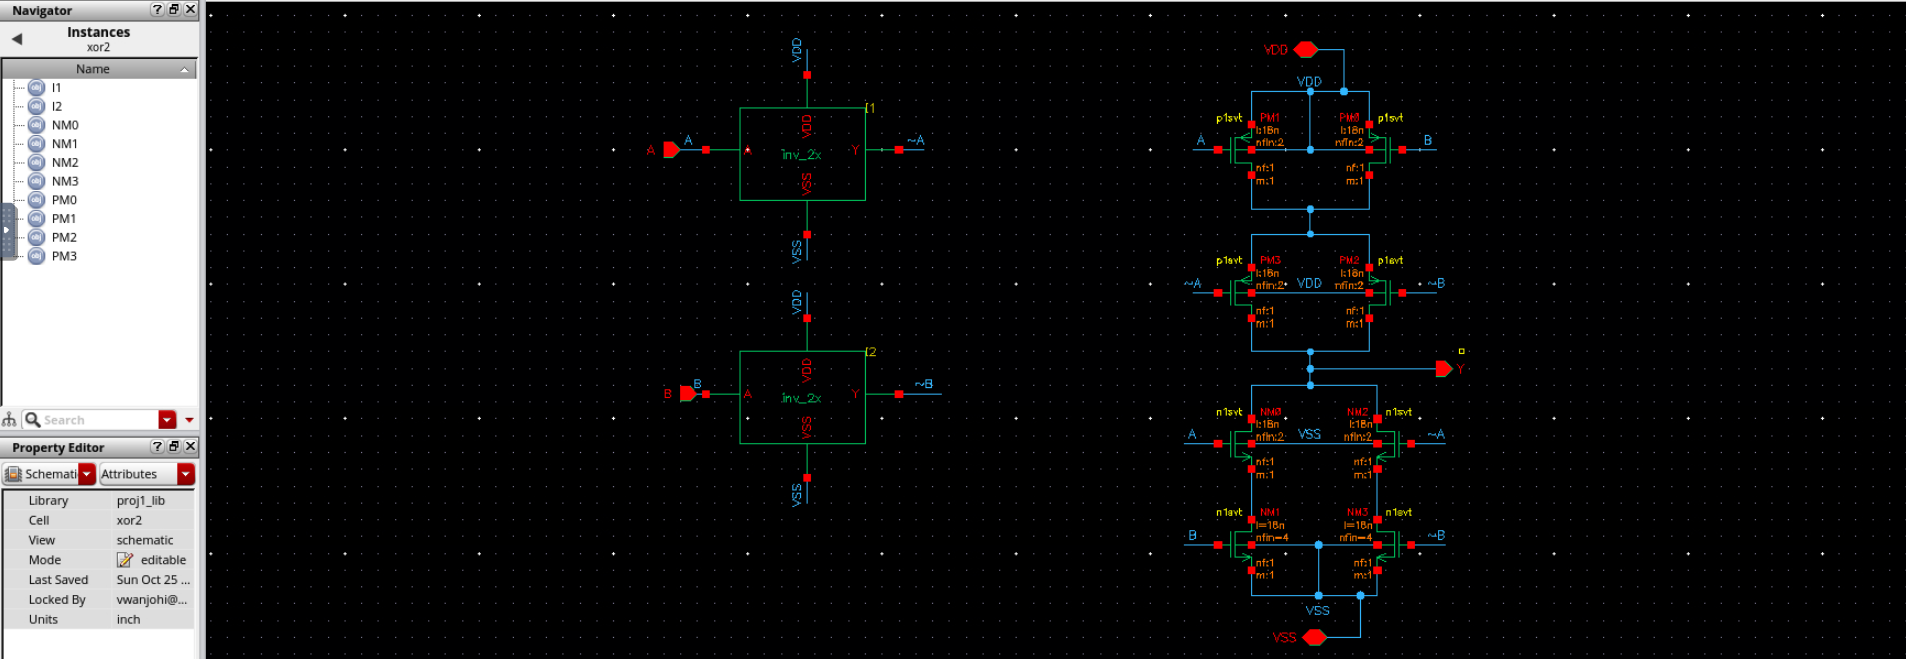
\includegraphics[width=.32\linewidth]{xor2_schematic}}{}\hfill
\IfFileExists{img/mux2_schematic.png}{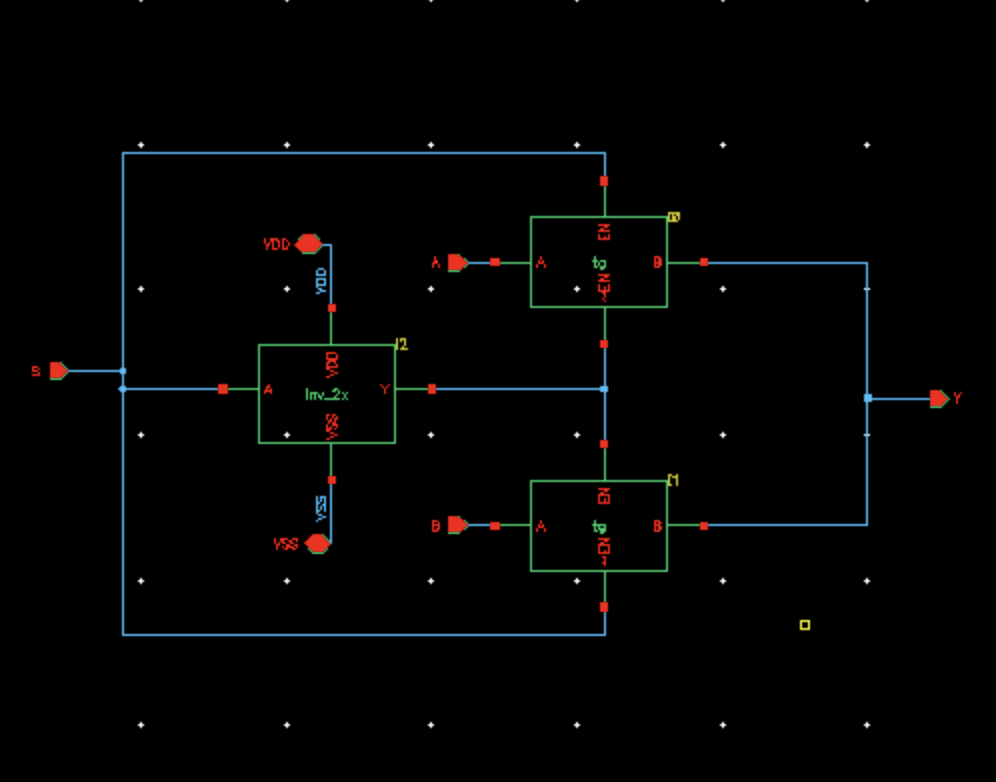
\includegraphics[width=.32\linewidth]{mux2_schematic}}{}
\caption{Leaf cells: \code{tg} (nfin 2 each), \code{xor2}, \code{mux2}. The \code{xor2} view is the corrected one (two series pull-down stacks). \todo{Re-capture \code{mux2} after the select swap.}}\end{figure}

\textbf{Multiplier.} Array multiplier: 16 AND gates form the partial products $a_ib_j$ (four \code{and2x4}, one per row $j$), and three 4-bit ripple-carry adders (\code{fulladder\_4b}, 12 full adders) sum the rows, each row shifted by one bit; $P_0=a_0b_0$, $P_{1..3}$ from the low bit of each adder row, $P_{4..7}$ from the last row and its carry. It reuses one verified full-adder cell in a regular array, which made it quick to build and debug; the cost is speed, because the longest path ripples through all three adder rows into the last row's carry ($P_6$, $P_7$). A carry-save (Wallace or Dadda) tree would shorten the path to two full-adder levels plus one final carry-propagate adder, for the same 12 full adders but irregular wiring. 2096 fins.
\fig{mult4x4_schematic}{.98}{\code{multiplier4b} (corrected): partial-product rows I4, I6, I8, I10 (\code{and2x4}, row $j$ gets $A\langle0..3\rangle$ and $B_j$ on all four B pins) and ripple rows I5, I7, I9 (\code{fulladder\_4b}, $C_{in}=0$); each row adds the previous row's upper sum bits and carry to the next partial product. Sizes ($L=18$ nm): \code{and2} $=$ \code{nand2\_u} (PMOS 2$\parallel$2, NMOS 2$+$2 series fins) $+$ \code{inv\_2x} (8/4); full adder: two \code{xor2} (NMOS 2/4, PMOS 2 fins, input \code{inv\_2x}), two \code{and2}, one \code{or2}.}

\textbf{Accumulator adder.} 12-bit ripple-carry adder of the same full adder (\code{fulladder\_12b}): $A=\mathrm{ACC}\langle11{:}0\rangle$, $B=\{0000,P\langle7{:}0\rangle\}$, $C_{in}=0$; the sum goes to \code{register\_12b} (12 \code{register\_1b}, $EN=$ ACC\_EN, synchronous reset on CLEAR). Twelve bits are enough: the largest result is $16\times15\times15=3600<4096$. Only the low 8 bits receive the product, so the upper 4 stages only propagate the carry. 3600 fins for the accumulator (1776 adder, 1824 register).
\fig{adder12_schematic}{.98}{\code{fulladder\_12b}: twelve \code{fulladder} cells in a ripple chain (I1 bit 0 with $C_{in}$ to I10 bit 11 with $C_{out}$), drawn as three rows of four; each cell is 148 fins (two \code{xor2}, two \code{and2}, one \code{or2}).}

\textbf{Logical-effort analysis (before simulation).} \todo{Path from the multiplier input (or register output) through the multiplier and adder to the accumulator register D pin.}
\begin{center}\small\begin{tabular}{@{}lllll@{}}\toprule Stage & Gate & $g$ & $p$ & Size / $h$\\\midrule
\todo{1} & & & & \\ \todo{\ldots} & & & & \\\midrule
\multicolumn{5}{@{}l}{Path effort $F=GBH=\todo{}$, $N=\todo{}$, $\hat f=F^{1/N}=\todo{}$, $D=N\hat f+P=\todo{}\,\tau$, $\tau=\todo{ps}$ (FO4 from Part 2) $\Rightarrow t_{\text{path}}\approx\todo{ps}$}\\\bottomrule\end{tabular}\end{center}

\textbf{Unit tests and predicted vs.\ measured.}
\begin{center}\small\begin{tabular}{@{}lllll@{}}\toprule Block & Bench & Test & Predicted delay & Measured delay\\\midrule
Multiplier & \code{tb\_multiplier} & Exhaustive: all 256 input pairs, product compared to $a\cdot b$ (error count must be 0); worst vector 182 ($A$ $5\to6$, $B=11$) & \todo{LE} & $>1.05$ ns \todo{rerun with stop $256\,t_v$}\\
12-bit accumulator & \code{tb\_accu\_12b} & \todo{accumulate, clear, hold; carry across all 12 bits (e.g.\ 0x0FF$+1$)} & \todo{} & \todo{}\\\bottomrule\end{tabular}\end{center}
\textbf{Multiplier bench} (\code{tb\_multiplier4b}, Fig.~below). Eight \code{vpulse} sources count through all 256 $(A,B)$ pairs, one per $t_v$ ($A$ the low nibble: bit $k$ has delay $2^k t_v$, width $2^k t_v$, period $2^{k+1}t_v$; $B$ bit $k$ uses $2^{k+4}t_v$), 20 ps edges, tran stop $256\,t_v$; each product bit drives one \code{inv\_2x} (\code{LD<7:0>}). \todo{Inputs are ideal sources; add two \code{inv\_u} buffers per input or state this.}
\fig{tb_multiplier4b_schematic}{.95}{\code{tb\_multiplier4b}. \todo{Re-capture with V8 $=$ \code{vdd} $=0.8$ V (this capture shows vdc $=1.8$) and V5 corrected to delay/width $32\,t_v$, period $64\,t_v$.}}
\fig{tb_multiplier4b_tran_A}{.95}{Stimulus $A\langle3{:}0\rangle$ at $t_v=1$ ns: $A_0$ toggles every vector, $A_3$ every 8.}
\fig{tb_multiplier4b_tran_B}{.95}{Stimulus $B\langle3{:}0\rangle$: $B$ steps once every 16 vectors, so all 256 pairs occur in 256 ns.}
\fig{tb_multiplier4b_tran_P_prefix}{.95}{First run (before the fixes): only $P_0=a_0b_0$ switches; $P_{1..7}$ stay near 0 V (mV-scale glitches). This located two design errors, below.}

\textbf{Errors found by the first run.} (1) \code{xor2}: the pull-down had the $A/\bar A$ devices in parallel, in series with the $B/\bar B$ pair in parallel, so it always conducted and fought the pull-up when $A\neq B$; corrected to two series stacks $A\cdot B$ and $\bar A\cdot\bar B$. (2) \code{multiplier4b}: all four \code{and2x4} received $(A\langle0..3\rangle, B\langle0..3\rangle)$ and formed $a_ib_i$; each row $j$ now receives $B_j$ on all four B inputs. A logic-level check of the corrected netlist gives 0 wrong products out of 256. \todo{Rerun: error count over 256 vectors, worst-case settling time from the $t_v$ sweep, delay of the slowest pair; replace the figure above with the passing run.}
\fig{tb_multiplier_tran}{.95}{After the fixes ($t_v=1$ ns): every product bit switches. First rising edges match the hand values: $P_1$ at vector 18 ($2\times1$), $P_3$ at 24 ($8\times1$), $P_4$ at 40 ($8\times2$), $P_5$ at 59 ($11\times3$), $P_7$ at 159 ($15\times9=135$); short spikes are ripple glitches inside a vector. \todo{Zoom on the worst-case transition.}}

\textbf{Exhaustive check.} Three ADE expressions turn the bits into integers: $P_{int}=\sum_k 2^k V(P_k)/V_{DD}$, $AB_{int}=(\sum_k 2^k V(A_k)/V_{DD})(\sum_k 2^k V(B_k)/V_{DD})$, and $\mathrm{err}=|P_{int}-AB_{int}|$. \code{errS} samples err once per vector at $0.95\,t_v$ (\code{sample(err, 0.95 tv, 255.95 tv, "linear", tv)}) and \code{errmax} $=$ \code{ymax(errS)} with spec $<0.5$.
\fig{tb_multiplier4b_err}{.95}{$P_{int}$ follows the $AB_{int}$ staircase in every block of 16 vectors; the err spikes sit at the vector boundaries, where $AB_{int}$ itself spikes because the input bits do not cross at the same instant.}
\fig{tb_multiplier4b_errS}{.95}{Sampled check at $t_v=1$ ns (top right, \code{errS}): 0 for almost all 256 vectors; about ten vectors in four clusters (56--60, 118--122, 180--185, 242--246 ns) are non-zero, peak \code{errmax} $=43.77$.}
At $t_v=1$ ns \code{errmax} $=43.77$ (71.45 with the earlier 0.9 $t_v$ sample point). The non-zero values are fractional, not the power-of-two error a settled wrong bit would give, so those vectors are still switching about 0.95 ns after the inputs: a settling limit, not a logic error.

\textbf{$t_v$ sweep (preliminary).} These sweeps ran with a fixed tran stop of 256 ns instead of $256\,t_v$, so for $t_v>1$ ns only the first $256\,\mathrm{ns}/t_v$ vectors were simulated (213 at 1.2 ns, 128 at 2 ns) and the last sample points fall after the end of the run. \todo{Rerun with stop time $256\,t_v$ and replace this table.}
\begin{center}\small\begin{tabular}{@{}rrrrl@{}}\toprule $t_v$ & sample point & \code{errmax} & \code{t\_worst} & reading\\\midrule
1.0 ns & 0.95 ns & 43.8 & 183.0 ns & fail, vector 182 ($A=6$, $B=11$), in range\\
1.1 ns & 1.045 ns & $\approx7.5$ & 201.2 ns & fail, vector 182 again, in range\\
1.2 ns & 1.14 ns & $\approx8.5$ & 256.7 ns & after the 256 ns stop: not valid\\
1.3 ns & 1.235 ns & $\approx0$ & 244.3 ns & pass for vectors 0--196 only\\
1.4, 1.5 ns & & $\approx0$ & 256.1, 238.4 ns & pass for the vectors simulated\\\bottomrule\end{tabular}\end{center}
The one solid result so far: the same vector, 182 ($A$: $5\to6$ at $B=11$, product $55\to66$), is the worst at both 1.0 and 1.1 ns and is still settling 1.045 ns after its edge, so the worst-case multiplier delay is above 1.05 ns. Typical vectors settle in 0.3--0.6 ns (zoom below). The residual 0.02--0.08 at long $t_v$ is the bit voltages sitting a few mV off the rails.
\fig{tb_multiplier4b_tv_sweep_fine}{.95}{Preliminary: \code{errmax} and \code{t\_worst} against $t_v$ (1.0--1.5 ns), fixed 256 ns stop. Points between sweep values are interpolated by the plot.}
\fig{tb_multiplier4b_tv_sweep_coarse}{.95}{Preliminary coarse sweep (1--4 ns, log axes), fixed 256 ns stop, so it covers only part of the 256 vectors for $t_v>1$ ns. (\code{errmax\_old} uses fixed 1 ns sample times and is not meaningful for $t_v\neq1$ ns.)}
\fig{tb_multiplier4b_zoom_tv1p2}{.95}{$P_{int}$ at $t_v=1.2$ ns, 233--256 ns ($B=12$, then $B=13$): each product settles 0.3--0.6 ns after its vector edge; the spike near 249.9 ns is the $180\to0$ step where all four $A$ bits and $B_0$ flip.}
\todo{Zoom on vector 182 at $t_v=1$ ns (200.2--201.2 ns window is vector 182 at 1.1 ns; at 1 ns it is 182--183 ns): which $P$ bit settles last, input-edge-to-0.4 V delay (the measured critical path for the logical-effort comparison).}
\fig{tb_accu_12b_tran}{.7}{\todo{Accumulator test, including the longest carry propagation.}}

%==============================================================
\section*{4. Sequencer (3.3)}
\rub{3.3}{4-bit address counter and control FSM (idle, compute, done) built from the registers; state diagram; timing of START, counter, memory reads, accumulator update and DONE over one dot product.}

\textbf{State diagram.}
\begin{center}
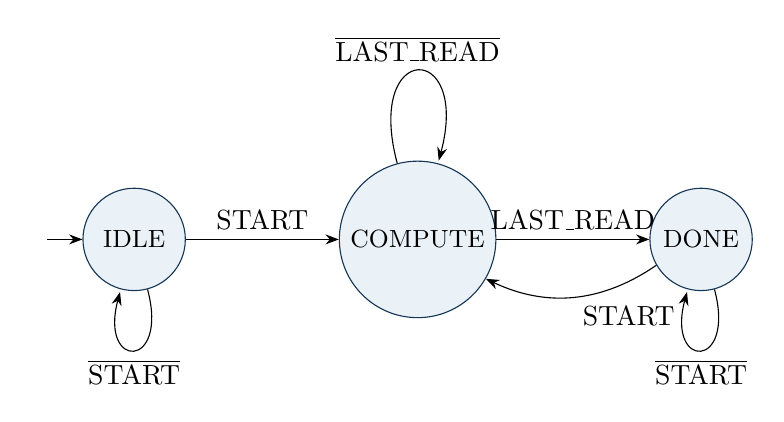
\begin{tikzpicture}[->,>=Stealth,node distance=3.6cm,auto,every state/.style={fill=pale,draw=navy,minimum size=1.3cm,font=\small}]
\node[state,initial,initial text=] (idle) {IDLE};
\node[state,right of=idle] (comp) {COMPUTE};
\node[state,right of=comp] (done) {DONE};
\path (idle) edge node {START} (comp)
      (comp) edge[loop above] node {$\overline{\mathrm{LAST\_READ}}$} ()
      (comp) edge node {LAST\_READ} (done)
      (done) edge[bend left=30] node {START} (comp)
      (idle) edge[loop below] node {$\overline{\mathrm{START}}$} ()
      (done) edge[loop below] node {$\overline{\mathrm{START}}$} ();
\end{tikzpicture}
\end{center}
Encoding (from \code{controller\_mac}): two state registers, $S_0$ and DONE; IDLE $=(S_0,\mathrm{DONE})=(0,0)$, COMPUTE: RUN $=S_0\overline{\mathrm{DONE}}=1$, DONE $=(0,1)$. Two more registers carry the pipeline: VALID ($=$ RUN one cycle late, so the first product is accumulated one cycle after its read) and LAST\_READ (set the cycle after the counter reaches 15). RST clears $S_0$ and DONE from any state. Per state:
\begin{itemize}\setlength{\itemsep}{0pt}\setlength{\topsep}{0pt}
\item \textbf{IDLE / DONE, START high:} $G_0=\mathrm{START}\cdot\overline{\mathrm{RUN}}$ raises CLEAR (clears the accumulator, the counter, VALID and LAST\_READ) and sets $S_0$; DONE clears. START is ignored while RUN.
\item \textbf{COMPUTE:} COUNT\_EN $=\mathrm{RUN}\cdot\overline{\mathrm{LAST}}$ steps the counter 0 to 15 and holds it at 15 (LAST $=$ count $=15$); ACC\_EN $=\mathrm{RUN}\cdot\mathrm{VALID}$; $S_0$ stays set while LAST\_READ $=0$.
\item \textbf{Leaving COMPUTE:} FINISH $=\mathrm{RUN}\cdot\mathrm{LAST\_READ}$ sets DONE and clears $S_0$, so the exit is one cycle after the count reaches 15, which leaves time to accumulate the last product.
\item \textbf{DONE:} held by $\mathrm{DONE}\cdot\overline{\mathrm{START}}$; ACC holds because ACC\_EN $=0$.
\end{itemize}

\textbf{Counter and controller.} \code{counter\_4b} is a synchronous toggle-chain counter: $T_1=EN\cdot Q_0$, $T_2=T_1Q_1$, $T_3=T_2Q_2$ (\code{and2}), $D_k=(Q_k\oplus T_k)\cdot\overline{RST}$ with $T_0=EN$ (\code{xor2}, \code{and2}), four \code{d\_ff}; RST is driven by CLEAR, so the count restarts at 0 on START (728 fins). \code{controller\_mac} is the logic above: 4 \code{register\_1b}, 11 \code{and2}, 3 \code{or2}, 5 \code{inv\_2x} (948 fins). In \code{top}, four \code{mux2} send COUNT to the memory address while RUN $=1$ and the external ADDR otherwise, and LOAD\_EN $=\overline{\mathrm{RUN}+\mathrm{DONE}+\mathrm{START}}$ gates WE\_W and WE\_X. \todo{\code{tb\_counter4b} and \code{tb\_controller} results (count 0 to 15 and wrap, hold, reset; START during compute ignored, DONE hold, restart from DONE).}
\fig{counter4b_schematic}{.98}{\code{counter\_4b}: four \code{d\_ff} (I5--I8); $D_k=(Q_k\oplus T_k)\cdot\overline{RST}$ through \code{xor2} and \code{and2} (I12/I13, I21/I22, I25/I26, I24/I23); toggle chain $T_1=EN\cdot Q_0$, $T_2=T_1Q_1$, $T_3=T_2Q_2$ (I15, I27, I28); RST inverted by I20. 728 fins.}
\fig{controller_schematic}{.48}{\todo{Controller.}}
\fig{tb_counter4b_tran}{.48}{\todo{Counter waveform.}}
\fig{tb_controller_tran}{.48}{\todo{Controller waveform.}}

\textbf{Timing over one dot product.} \todo{Annotated diagram, as in Part 2 (\code{timing\_diagram\_2p2c.tex} is the model): CLK, START, state, counter, ADDR to the macros, $W$/$X$ outputs, product, ACC, DONE; mark the START edge, the first read, the first accumulate, the last accumulate, DONE rising.}
\begin{center}\small\begin{tabular}{@{}ll@{}}\toprule Architecture & pipelined: address and read in cycle $n$, multiply-accumulate in $n+1$ (VALID)\\
Cycles START to DONE & 17 edges after the START edge (cycle-level model of the netlist; limit 20) \todo{confirm in \code{tb\_top}}\\
Cycles per dot product & 17 (plus 32 load cycles when the memories are reloaded)\\\bottomrule\end{tabular}\end{center}

%==============================================================
\section*{5. Timing closure (3.4)}
\rub{3.4}{critical path identified; minimum period by hand from $t_{CLK\to Q}$/SRAM access, the logical-effort datapath estimate, and register $t_{cq}$ and $t_{su}$; measured as the shortest passing period; hold checked on fast paths.}

\textbf{Critical path.} The pipeline has no register between the macros and the multiplier: the macro's own address latch captures COUNT at the rising edge and its output latch holds DOUT for the rest of the cycle. The paths that must fit in one period are therefore (1) counter $t_{cq}$ $\to$ \code{mux2} $\to$ macro address latch (short), and (2) CLK edge $\to$ SRAM access $\to$ multiplier $\to$ 12-bit adder $\to$ accumulator setup, the critical path: $T_{\min}\ge t_{\text{SRAM}}+t_{\text{mult}}+t_{\text{add}}+t_{su}$, with $t_{\text{SRAM}}$ measured from CLK and so already including the macro's internal address latch.
\begin{equation}
T_{\min}\ge t_{cq}+t_{\text{SRAM}}+t_{\text{mult}}+t_{\text{add}}+t_{su}+t_{\text{skew}}\quad\text{(non-pipelined)};\qquad
T_{\min}\ge\max\bigl(t_{cq}+t_{\text{SRAM}}+t_{su},\ t_{cq}+t_{\text{mult}}+t_{\text{add}}+t_{su}\bigr)\quad\text{(pipelined)}.
\end{equation}
\begin{center}\small\begin{tabular}{@{}lll@{}}\toprule Term & Value & Source\\\midrule
$t_{cq}$ (register) & \todo{ps} & \S2\\
$t_{\text{SRAM}}$ (CLK to DOUT) & 488 ps & Part 2, worst case at $T_{CLK}=0.69$ ns\\
$t_{\text{mult}}+t_{\text{add}}$ & $t_{\text{mult}}>1050$ ps measured; \todo{LE estimate, $t_{\text{add}}$} & \S3\\
$t_{su}$ & \todo{ps} & \S2\\\midrule
\textbf{Hand $T_{\min}$} & \todo{ns} & sum\\
\textbf{Measured $T_{\min}$} & \todo{ns} & shortest period at which tests A, B, C pass (resolution \todo{10 ps})\\\bottomrule\end{tabular}\end{center}

\textbf{Period sweep.} \todo{Table as in Part 2 \S6: $t_{clk}$, ACC error for A/B/C, result.} Discuss the gap between hand and measured value: \todo{}.
\fig{tb_top_tclk_sweep}{.7}{\todo{Pass/fail against clock period.}}

\textbf{Hold check at the fast paths.} Two short paths: (1) counter $\to$ \code{mux2} $\to$ macro address latch, which closes at the same rising edge that changes the counter, so the new count must arrive after the latch has closed: $t_{cq,\min}+t_{\text{mux}}\ge t_{h,\text{latch}}$; (2) register to register in the controller and counter (e.g.\ VALID from RUN through one \code{and2}): $t_{cq,\min}+t_{\text{logic,min}}\ge t_h+t_{\text{skew}}$. \todo{Margins in ps from \code{tb\_dff} ($t_{cq,\min}$, $t_h$) and a simulation of path (1) in \code{tb\_top}.}

%==============================================================
\section*{6. Verification (3.5)}
\rub{3.5}{three test vectors; ACC and DONE waveforms for Test A; pass/fail table for all three.}

\textbf{Bench} (\code{tb\_top}). \todo{Load phase: START low, WE\_W/WE\_X write 16 words each through ADDR/DIN, one per cycle; compute phase: START pulse, wait for DONE, sample ACC. Inputs through realistic buffers as in Part 2. ACC compared to the expected value with an error measure.}

\begin{center}\small\begin{tabular}{@{}p{.12\linewidth}p{.33\linewidth}p{.33\linewidth}l@{}}\toprule Test & $W[0..15]$ & $X[0..15]$ & Expected ACC\\\midrule
A & 3, 12, 7, 0, 15, 9, 1, 14, 6, 11, 2, 13, 8, 5, 10, 4 & 9, 2, 15, 7, 4, 12, 0, 11, 13, 1, 8, 6, 3, 14, 5, 10 & 845 (0x34D)\\
B & all 15 & all 15 & 3600 (0xE10)\\
C & 5, 10, 5, 10, \ldots & 10, 5, 10, 5, \ldots & 800 (0x320)\\\bottomrule\end{tabular}\end{center}

\begin{center}\small\begin{tabular}{@{}lllllll@{}}\toprule Test & Expected & ACC read & DONE high at cycle & Cycles & Result\\\midrule
A & 845 (0x34D) & \todo{} & \todo{} & \todo{} & \todo{pass/fail}\\
B & 3600 (0xE10) & \todo{} & \todo{} & \todo{} & \todo{}\\
C & 800 (0x320) & \todo{} & \todo{} & \todo{} & \todo{}\\\bottomrule\end{tabular}\end{center}
Test B is the full-scale case (largest carry chains, no overflow); Test C alternates $5\times10$ and $10\times5$ to maximize toggling on the memory outputs and multiplier inputs.

\fig{tb_top_testA_acc_done}{.9}{\todo{Test A: ACC$\langle11{:}0\rangle$ as a bus and DONE; mark START, first accumulate, DONE rising, final value 0x34D, and that ACC holds until the next START.}}
\fig{tb_top_testA_partial_sums}{.7}{\todo{Optional: running partial sums against the hand-computed values for Test A.}}
\todo{Also check, if time allows: RST mid-computation, START during compute, back-to-back dot products without reloading (ACC clears on START).}

%==============================================================
\section*{7. Metrics and figure of merit}
\rub{handout}{$T_{CLK,\min}$ and $t_{dot}=N_{cycles}\cdot T_{CLK,\min}$ (START to DONE); $E_{dot}$ = supply energy from START to DONE at $T_{CLK,\min}$ for Test A, also B and C, split into memory, datapath, sequencer if separate supplies; area = 2 macros (Part 2) + datapath and sequencer with $D$; FOM$_{MAC}$ = Area $\cdot E_{dot}\cdot t_{dot}$ ($\mu$m$^2$, pJ, ns); energy per MAC with and without the memory accesses; paragraph on where the energy goes.}

At $V_{DD}=0.8$ V, nominal, 27$^\circ$C, $D=28$:
\begin{center}\small\begin{tabular}{@{}p{.4\linewidth}p{.56\linewidth}@{}}\toprule Metric & Value\\\midrule
$T_{CLK,\min}$ & \todo{ns} (measured); hand estimate \todo{ns}\\
$N_{cycles}$ (START to DONE) & 17 (predicted) \todo{confirm}\\
$t_{dot}=N_{cycles}\,T_{CLK,\min}$ & \todo{ns}\\
Area: 2 macros $+$ datapath $+$ sequencer & $2\times54.6$ \est\ $+\ D\sum W_iL_i$ (7544 fins $\times\ 0.0242\ \mu$m$^2$: datapath 5696 fins $=137.8$, sequencer and glue 1848 fins $=44.7$) $=\mathbf{291.8\ \mu}$\textbf{m}$^\mathbf{2}$ \est\\
\textbf{FOM$_{MAC}$ $=$ Area$\cdot E_{dot}\cdot t_{dot}$} (Test A) & \todo{$\mu$m$^2\cdot$pJ$\cdot$ns}\\\bottomrule\end{tabular}\end{center}

\textbf{Energy} (integral of supply current $\times V_{DD}$ from START to DONE, at $T_{CLK,\min}$):
\begin{center}\small\begin{tabular}{@{}lllll@{}}\toprule Test & $E_{dot}$ total & Memory (2 macros) & Datapath & Sequencer\\\midrule
A & \todo{pJ} & \todo{} & \todo{} & \todo{}\\
B (all 15) & \todo{pJ} & \todo{} & \todo{} & \todo{}\\
C (5/10 alternating) & \todo{pJ} & \todo{} & \todo{} & \todo{}\\\bottomrule\end{tabular}\end{center}
\todo{State how the split is obtained (separate supply sources per block, with the registers counted in the block they belong to).}
\begin{center}\small\begin{tabular}{@{}lll@{}}\toprule & With memory accesses & Without memory accesses\\\midrule
Energy per MAC, Test A ($E_{dot}/16$) & \todo{pJ} & \todo{pJ}\\\bottomrule\end{tabular}\end{center}
\textbf{Where the energy goes.} \todo{Paragraph: share of memory against datapath and sequencer; clock tree and register energy per clock (\S2) times the number of registers; why B and C differ from A (toggling); static versus dynamic.}

%==============================================================
\section*{8. What limited the design}
The clock period is set by the multiply-accumulate path, not the memory: the array multiplier alone takes more than 1.05 ns in its worst case, over twice the 488 ps SRAM read, before the 12-bit ripple adder and the register setup are added. Both arithmetic blocks are ripple structures built from one small full adder (2-fin \code{xor2} stacks with input inverters), which made them easy to verify but long. In area the datapath (138 $\mu$m$^2$) is larger than the two macros (109 $\mu$m$^2$ \est), mostly the 24 full adders and the 12 accumulator registers. \todo{Energy split once measured.} With more time: a carry-save multiplier, a faster final adder (carry-select or lookahead), upsized \code{xor2} stacks, and a pipeline register after the multiplier.
\begin{itemize}\setlength{\itemsep}{0pt}\setlength{\topsep}{0pt}
\item \textbf{Register style:} static TG master-slave, 100 fins per flip-flop (152 with enable and reset), reused everywhere; a dynamic latch would be smaller and faster but cannot hold with the clock stopped. \todo{$t_{cq}$, $t_{su}$, energy per clock.}
\item \textbf{Pipelined vs.\ not:} overlapping the read with the multiply-accumulate costs one cycle (17 instead of 16) and stays within the 20-cycle limit; because the macro output latch is the only pipeline stage, the SRAM access and the arithmetic still share one period. A register after the multiplier would split them, at a second extra cycle (18).
\item \textbf{Multiplier and adder architecture:} ripple array and ripple adder: smallest design effort and regular, but the slowest choice; a carry-save tree and a carry-select final adder are the first changes for speed.
\end{itemize}
\end{document}
